\begin{figure}[htb]
    \centering

    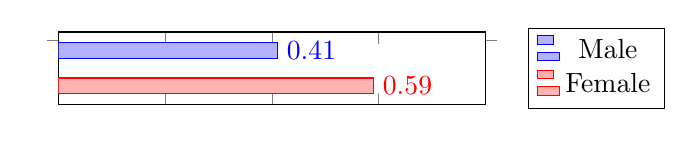
\begin{tikzpicture}
        \begin{axis}[
            xbar, xmin=0, xmax=0.8,
            width=7cm,height=2.5cm,
            bar width=2mm,
            symbolic y coords={F,M},
            ytick=data,enlarge y limits={abs=1mm},
            nodes near coords,
            yticklabels={,},
            xticklabels={,},
            legend style={
                at={(1.1,0.5)},
                anchor=west,
            }
        ]
            \addplot coordinates { (0.41,{M}) };
            \addplot coordinates { (0.59,{F}) };
            \legend{Male, Female}
        \end{axis}
    \end{tikzpicture}
    \caption{Sex Distribution}

\end{figure}